\chapter{Financial Projections}

In Joseph Hadzima's MIT OpenCourseWare course, Steve Durzynski takes over just after the financing panel and asks the next unavoidable question: once we know the customer, the business model, the team, and the legal form, what resources does the venture actually need in order to live? This companion chapter, curated by LazyingArt LLC, follows that sequence closely. We begin with the claim that cash is the venture's oxygen; then we move through investor arithmetic, the grammar of the standard financial statements, the bottom-up construction of a model, the four-year profit-and-loss view, the quarterly cash-flow recurrence, and only then the late turn to equity, dilution, vesting, and control. The lecture's central discipline is simple to state and hard to avoid: the model is not a ceremonial prediction, but a machine for forcing our assumptions into the open.

\section{Why We Need Financial Projections}

The lecture begins by confronting a founder's natural impatience. We are busy building the product, finding customers, hiring people, and keeping the team together. Why stop for a spreadsheet that will be wrong anyway? Durzynski does not deny the objection. He answers it by changing the meaning of the exercise. Financial projection is not introduced as bureaucratic accounting; it is introduced as operational survival.

His governing metaphor is exact and memorable: cash is the oxygen of the venture. We can live without many things for a while, but not without oxygen. Once that point is accepted, the model ceases to be decorative. It becomes the scorecard for the firm's condition, the roadmap for future spending, and the instrument by which outside money is obtained. An investor, banker, or financial advisor is not only asking whether the upside is large. They are asking whether the founder understands the structure of the business well enough to see the downside, the cash needs, the milestones, and the risks.

A compact way to express the operating pressure is through burn:
\begin{equation}
\mathrm{BurnRate} = \mathrm{MonthlyOperatingLoss} + \mathrm{CapitalExpenditures}.
\end{equation}
This is not yet formal accounting, but it is already managerial arithmetic. Once we know what we lose each month and what capital equipment we must buy, we are much closer to the real question: how long can we keep breathing?

The lecture is equally insistent that this understanding cannot be outsourced in any meaningful sense. One may hire accountants and later bring in a CFO, but at the beginning the founder has to develop a direct feel for the business. Where does the money go? Which hires matter first? What is the average selling price? How expensive is customer acquisition? Which milestone, if delayed, throws the whole plan off? The spreadsheet is valuable precisely because it forces us to ask these questions in an organized form.

\section{Investor Arithmetic Before Accounting}

Before Durzynski teaches the grammar of financial statements, he gives the class the arithmetic of venture capital. This is the right order. We first want to know what sort of outcome a venture-backed company must plausibly support. Only then do we ask how the internal model should be built.

A venture fund has its own obligations to its limited partners. That is why not every good business is venture fundable. A company that grows too slowly may be a perfectly respectable business for its founders and still fail the venture test. The point is not moral; it is arithmetic. Durzynski gives the lecture's clean rule of thumb:
\begin{equation}
(1+r)^5 = 4
\qquad \Rightarrow \qquad
r \approx 0.32.
\end{equation}
A four-times return in five years corresponds to an internal rate of return of roughly \(32\%\). One should read this as a heuristic from the lecture, not as a law of nature, but it is enough to show why the slope of the expected curve matters.

The ownership formula is then stated in its simplest form. If an investor puts in \(I\) dollars at a pre-money valuation \(V_{\mathrm{pre}}\), the post-money valuation is
\begin{equation}
V_{\mathrm{post}} = V_{\mathrm{pre}} + I,
\end{equation}
and the fraction sold in that round is
\begin{equation}
f = \frac{I}{V_{\mathrm{pre}} + I}.
\end{equation}

\paragraph{Worked example.}
If we raise \(\$1\text{M}\) at a \(\$4\text{M}\) pre-money valuation, then
\begin{equation}
f = \frac{1}{4+1} = \frac{1}{5} = 20\%.
\end{equation}
The investor owns one-fifth of the company after the round, and the post-money valuation is \(\$5\text{M}\).

Durzynski then gives a two-round example, because ownership is only the beginning; dilution is the real story:
\begin{align}
f_A &= \frac{5}{5+5} = 50\%, \\
f_B &= \frac{10}{15+10} = 40\%.
\end{align}
The second round dilutes the holders from the first round. If the first investor had \(50\%\), then after a new \(40\%\) round that stake becomes
\begin{align}
\omega_{A,\mathrm{after}\ B} &= 0.50(1-0.40)=0.30, \\
\omega_{\mathrm{VC,total}} &= 0.30 + 0.40 = 0.70.
\end{align}
So after these two rounds the venture investors together own about \(70\%\) of the company.

At this point the lecture makes its crucial move. The problem is no longer only dilution; it is scale. If investors have put in \(\$15\text{M}\) and want something like \(4\times\) to \(6\times\) back, then their stake must eventually be worth roughly \(\$60\text{M}\) to \(\$90\text{M}\). Using the lecture's \(70\%\) ownership figure, the implied exit value is on the order of
\begin{equation}
V_{\mathrm{exit}} \approx \frac{60\text{M}}{0.70}\ \text{to}\ \frac{90\text{M}}{0.70}
\approx 86\text{M to }129\text{M}.
\end{equation}
The transcript is garbled around the exact spoken figure, so this should be read as cautious reconstruction. The important point is not the last digit. The important point is that once we raise substantial capital, the required exit and revenue scale move upward with it.

\subsection{Question \& Answer}

\paragraph{Question.}
If raising money sounds like success, why does it also make success harder?

\paragraph{Answer.}
Because the new money buys runway but also installs a larger claim on the future. The round does not merely validate the company; it raises the minimum outcome that will count as a successful venture return. A press release may celebrate \(\$5\text{M}\) raised, but financially the better question is: what revenue and exit value must now be achieved in order for that capital to have been worth taking? The lecture's warning is that each new round can lower risk locally while raising the bar globally.

\section{Reading the Business Through Standard Financials}

Only now do we get the standard set of financial statements. This order matters. The lecturer wants us to see accounting not as a separate discipline but as the language in which the operational story becomes visible.

\paragraph{Income statement.}
The income statement, or profit-and-loss statement, is the one everyone thinks they know. We sell something, subtract what it costs to produce, and look at what remains. In compact form:
\begin{align}
\mathrm{GrossMargin}_t &= R_t - \mathrm{COGS}_t, \\
\mathrm{OperatingProfit}_t &= R_t - \mathrm{COGS}_t - \mathrm{DeptExp}_t.
\end{align}
Here \(R_t\) is revenue, \(\mathrm{COGS}_t\) is cost of goods sold, and \(\mathrm{DeptExp}_t\) is the rollup of departmental expenses such as sales, marketing, R\&D, G\&A, staffing, and the rest of the operating structure.

\paragraph{Balance sheet.}
The balance sheet holds assets, liabilities, and equity. Cash is an asset, but so are patents, equipment, and other property. Debt sits on the liability side. Equity is the residual claim. This matters later when the lecture pivots to the cap table, because share ownership belongs to the balance-sheet side of the story, not to the revenue line.

\paragraph{Cash-flow statement.}
The cash-flow statement is where money actually enters and leaves. Durzynski treats it visually rather than doctrinally: money comes in, money goes out, and the level rises and falls. That is enough to see why profit alone is not the same as survival.

The lecture then shifts from absolute dollars to percentages. This is a subtle but important step. Boards and investors often compare firms through normalized ratios rather than raw totals. The reason is straightforward: absolute size varies wildly, but the percentage signature of a business model is often recognizable. We therefore define
\begin{equation}
\mathrm{GrossMarginPct}_t = \frac{\mathrm{GrossMargin}_t}{R_t},
\qquad
\mathrm{OpMargin}_t = \frac{\mathrm{OperatingProfit}_t}{R_t}.
\end{equation}
Different businesses leave different ratio fingerprints.

The old-school hardware and software comparisons serve exactly this purpose. A hardware company with very low R\&D and low operating margin tells one story; a software company with higher R\&D, higher SG\&A, and higher eventual margins tells another. Joe Hadzima's interjection sharpens the logic: if our projected ratios differ greatly from those of successful comparable businesses, then we must either explain the difference by a genuinely different business model or accept that the model lacks credibility.

This is why the lecture treats year-four ratios as more useful than year-one ratios. Early startup years are noisy and often loss-making. But by the year-four view, we should begin to see something structurally recognizable. The lecture gives rule-of-thumb targets of roughly \(10\%\) to \(20\%\) for R\&D as a fraction of revenue, roughly \(5\%\) to \(15\%\) for G\&A, and roughly \(15\%\) to \(20\%\) for operating profit. These are not identities. They are comparison standards.

\section{Building the Model From the Bottom Up}

Once the class has the grammar, the lecture turns to construction. Here the tone changes. We are no longer merely reading a business; we are assembling one.

The model begins with concrete questions. What is the product or service? What price can it command? What does it cost to manufacture or deliver? What overhead is needed to support it? How will it be sold: directly, through distributors, through partners, through a founder-led process, or through a later sales force?

One of the lecture's cleanest small examples contrasts direct sale and distributor sale. If the nominal sale price is \(100\), then in the direct case the company books the full sale price as revenue:
\begin{equation}
\mathrm{BookedRevenue}_{\mathrm{direct}} = 100.
\end{equation}
In the distributor case, the distributor may take \(20\) off the top, so the company books
\begin{equation}
\mathrm{BookedRevenue}_{\mathrm{distributor}} = 100 - 20 = 80.
\end{equation}
The tradeoff is immediate. Revenue booked is lower, but the selling burden may also be lower. This is exactly the kind of high-level strategic choice that changes the financial structure.

The lecture also insists that in early stages the founders are often the first salespeople. That point is more than anecdotal. It means the model cannot jump magically from zero to scale. We have to ask how the first customer is obtained, then the second, then the tenth. We must ask how long the sales cycle is, whether there are support contracts that renew, how much marketing spend is required, and how quickly new salespeople become productive.

The staffing side enters next, because staffing usually drives departmental expense. The lecture's rules of thumb are deliberately practical:
\begin{equation}
\mathrm{Benefits} \approx 0.15 \times \mathrm{Salary},
\qquad
\mathrm{DeptExp}_{\mathrm{staff}} \approx 0.67 \times \mathrm{TotalExpenses}.
\end{equation}
Again, these are heuristics, not laws. But they force the right scale of thinking. Most early cash burn goes into people.

This leads naturally to one of the lecture's more human financial principles: founder salary should be minimum viable salary. The founder should not starve, but should not use newly raised money as personal extraction. The large payoff, in this framework, is meant to sit in equity, not salary.

The same bottom-up realism governs the sales forecast. The model should be built from one customer to two to many, not from fantasy market-share arithmetic. Yet the lecture adds a necessary corrective: bottom-up does not mean blind. A sanity check against market size is still required. If our bottom-up forecast implies owning more than the whole market, then the model has failed.

Durzynski is equally sharp about tools. Business-planning software is not recommended as a substitute for understanding, and AI is treated cautiously. It may help generate ideas about metrics or strategy, but the founder still needs to own the cells, the assumptions, and the consequences. A model we cannot defend is not our model.

\subsection{Question \& Answer}

\paragraph{Question.}
Why is a bottom-up sales forecast more credible than a large market-share story?

\paragraph{Answer.}
Because a bottom-up forecast exposes mechanism. It forces us to say who buys, at what price, through which channel, on what timetable, with what staffing, and at what cost. A large-market story usually hides all of that beneath a percentage of an enormous total. Investors do not fund market size; they fund sales machinery. A defendable forecast is one whose gears can be named.

\section{From Assumptions to the Four-Year P\&L}

At this point the lecture makes a strong methodological move: start with the end in mind. Instead of walking first through every worksheet tab, Durzynski shows the finished four-year profit-and-loss output. This is not a shortcut. It is a teaching device. He wants us first to see the shape of the destination.

\begin{figure}[t]
\centering

\includegraphics[width=0.96\linewidth]{lecture_08_figure_02.png}
\caption{Four-year P\&L forecast with revenue and operating profit.}
\end{figure}

The slide is visually clear. Revenue rises sharply from year to year. Operating profit begins below zero, crosses the horizontal axis after Year 2, and continues upward thereafter. The point is not precision of the plotted coordinates; the point is the geometry of a plausible startup path. Loss comes first, then break-even, then operating leverage.

\begin{figure}[t]
\centering
\begin{tikzpicture}[x=1.9cm,y=0.11cm]
\draw[->] (0,-28) -- (0,80);
\draw[->] (0,0) -- (4.4,0);

\draw (0,-25) -- (4.0,-25);
\draw (0,25) -- (4.0,25);
\draw (0,50) -- (4.0,50);
\draw (0,75) -- (4.0,75);

\node[anchor=east] at (-0.1,-25) {$-25$};
\node[anchor=east] at (-0.1,0) {$0$};
\node[anchor=east] at (-0.1,25) {$25$};
\node[anchor=east] at (-0.1,50) {$50$};
\node[anchor=east] at (-0.1,75) {$75$};

\node at (0.8,-31) {Year 1};
\node at (1.8,-31) {Year 2};
\node at (2.8,-31) {Year 3};
\node at (3.8,-31) {Year 4};

\draw[thick,red] (0.8,2) -- (1.8,12) -- (2.8,38) -- (3.8,66);
\draw[thick,blue] (0.8,-4) -- (1.8,-2) -- (2.8,7) -- (3.8,16);

\node[anchor=west] at (3.9,66) {Revenue};
\node[anchor=west] at (3.9,16) {Operating Profit};
\end{tikzpicture}
\caption{Qualitative redraw of the four-year forecast. The geometry is schematic rather than numerically exact.}
\end{figure}

This picture allows the lecturer to make a very useful inference. If we sum the negative operating results before break-even, we estimate how much cash the company needs in order to survive until profitability. The lecture gives a concrete version of that arithmetic:
\begin{equation}
\mathrm{CashNeed}_{\mathrm{pre\mbox{-}BE}} \approx 3.3\text{M} + 2.6\text{M}
\approx 5.9\text{M} \approx 6\text{M}.
\end{equation}
The graph suggests the same thing in a more geometric language:
\begin{equation}
\mathrm{CashNeed}_{\mathrm{pre\mbox{-}BE}}
\approx
\int_{\mathrm{OperatingProfit}(t)<0}
-\mathrm{OperatingProfit}(t)\,dt.
\end{equation}
The lecture uses this only as a visual intuition -- an ``integral under the curve'' way of thinking -- not as a claim that the chart itself gives precise continuous data. But the conceptual move is excellent. The losses before break-even are not incidental; they are the cash burden that must be financed.

That is why Durzynski says that even if the curve suggests roughly \(\$6\text{M}\) of need, one should probably raise more, perhaps \(\$10\text{M}\), so there is room for mistakes, delays, and surprises. The model is not only an argument for future profitability. It is an estimate of how much uncertainty the firm can survive.

The lecturer also glances at the slope of the revenue line and uses it as a rough visual indicator of growth quality. The transcript is unstable around the word he uses there, and one should not formalize it too aggressively. The safe point is that the chart is read not only for sign changes, but for the steepness of the venture's scale-up.

\subsection{Question \& Answer}

\paragraph{Question.}
If the company loses money in the first years, what exactly makes the model credible?

\paragraph{Answer.}
Not the smoothness of the graph by itself. Credibility comes from the path underneath the graph: units sold, selling price, channel choice, support retention, manufacturing cost, hiring plan, rent, overhead, and timing. The early losses are acceptable only if the route from those losses to later profitability can be explained in operational detail. The graph compresses the story; it does not replace the story.

\section{Cash Flow, CAPEX, and the Timing of Survival}

After the annual and quarterly P\&L rollups, the lecture turns to the cash-flow view. This is where the model stops being merely descriptive and becomes dynamic. We no longer ask only whether the business looks profitable eventually. We ask when cash actually runs low, and when the next financing must occur.

\begin{figure}[t]
\centering

\includegraphics[width=0.96\linewidth]{lecture_08_figure_03.png}
\caption{CAPEX and cash-flow spreadsheet layout.}
\end{figure}

The slide teaches several things at once. First, it shows the row order of the cash model: beginning cash, investment, revenue, costs, capital expense, change in cash, ending balance. Second, it shows that the workbook is modular: the lower capital-expense table feeds the upper cash-flow table, while other tabs feed both. Third, it teaches the color semantics of the spreadsheet itself: red means user input, magenta means link to another sheet, black means calculated value, and blue means value pulled in from another sheet.

The core recurrence can be written cleanly as
\begin{align}
\Delta C_q &= I_q + R_q - \mathrm{COGS}_q - \mathrm{DeptExp}_q - \mathrm{CapEx}_q, \\
C_q^{\mathrm{end}} &= C_q^{\mathrm{beg}} + \Delta C_q, \\
C_{q+1}^{\mathrm{beg}} &= C_q^{\mathrm{end}}.
\end{align}
This is the bookkeeping spine of the slide. One begins the quarter with cash, adds financing and revenue, subtracts costs and capital spending, and carries the remainder into the next quarter.

The lower table provides the capital-expense side of this recurrence. In abstract form,
\begin{equation}
\mathrm{CumCapEx}_q = \sum_{\tau \le q} \mathrm{CapEx}_{\tau}.
\end{equation}
The screenshot also makes clear that the capital line is not mysterious. It is fed from concrete items such as employee workstations and prototype expense.

\begin{figure}[t]
\centering
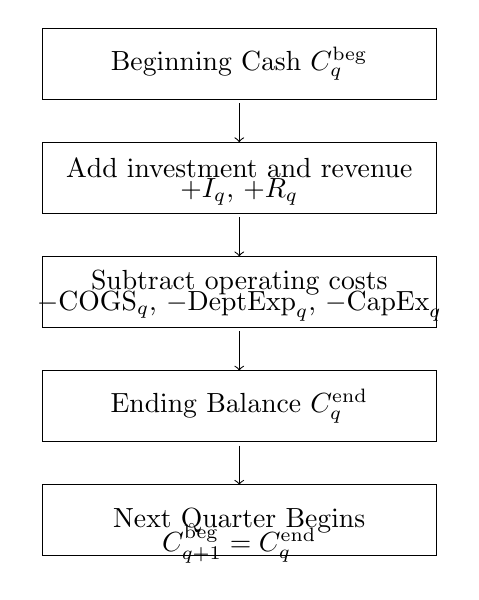
\begin{tikzpicture}[x=1cm,y=1cm]
\draw (0,0) rectangle (5,0.9);
\node at (2.5,0.45) {Beginning Cash $C_q^{\mathrm{beg}}$};

\draw[->] (2.5,-0.05) -- (2.5,-0.55);

\draw (0,-1.45) rectangle (5,-0.55);
\node at (2.5,-0.88) {Add investment and revenue};
\node at (2.5,-1.18) {$+I_q$, $+R_q$};

\draw[->] (2.5,-1.5) -- (2.5,-2.0);

\draw (0,-2.9) rectangle (5,-2.0);
\node at (2.5,-2.33) {Subtract operating costs};
\node at (2.5,-2.63) {$-\mathrm{COGS}_q$, $-\mathrm{DeptExp}_q$, $-\mathrm{CapEx}_q$};

\draw[->] (2.5,-2.95) -- (2.5,-3.45);

\draw (0,-4.35) rectangle (5,-3.45);
\node at (2.5,-3.90) {Ending Balance $C_q^{\mathrm{end}}$};

\draw[->] (2.5,-4.40) -- (2.5,-4.90);

\draw (0,-5.80) rectangle (5,-4.90);
\node at (2.5,-5.35) {Next Quarter Begins};
\node at (2.5,-5.65) {$C_{q+1}^{\mathrm{beg}} = C_q^{\mathrm{end}}$};
\end{tikzpicture}
\caption{Cash-flow recurrence implied by the workbook structure.}
\end{figure}

Durzynski's spoken walkthrough makes the recurrence concrete. Start with zero. Add \(\$5\text{M}\) of investment. Spend through the quarter. End with roughly \(\$4\text{M}\). Carry that amount forward as the next quarter's beginning cash. Spend again. If the balance falls toward a dangerous floor, then the timing of the next raise becomes visible. In the lecture's example, that means raising more money before the cash level drops below a comfortable threshold.

This is why cash flow is operationally more valuable than many founders first assume. Some conversations will focus on the income statement, especially at high level. But when the question becomes survival, the cash-flow statement is where timing enters the analysis. Survival is not only about whether the business can make money in the long run. It is about whether the firm can stay alive long enough to reach the long run.

\section{Presentation Discipline and the Late Pivot to Equity}

Once the model exists, the lecture asks how it should be presented. The first principle is that the model is iterative. It should be beaten up by friends, by mentors, and by investors in due diligence. The point of that pressure is not humiliation. The point is to discover the weak assumptions while there is still time to repair them.

At the executive-summary level, the lecture recommends an annual P\&L view with percentages, so that investors can pattern-match the business quickly. In deeper diligence, one may need the full structure: annual P\&L, quarterly P\&L, staffing plan, quarterly cash flow, and the assumptions behind pricing, hires, milestones, and profit timing. The large venture firm may even bring in its own finance professional to push on the weak points.

The lecture is also disciplined about risk presentation. One should know the major risks and have mitigations ready. But one should not lead the pitch with best-case and worst-case scenarios. Those belong more naturally in backup material or in the appendix, especially when the founder is controlling the presentation. The founder is asked to show conviction in a single base case and then defend it under questioning.

Only after this financial spine is built does Durzynski pivot to equity. This ordering is correct. The pie is not split in a vacuum; it is split after we understand what sort of enterprise is being financed.

The algebra of the cap table is simple:
\begin{equation}
\omega_i = \frac{s_i}{S},
\end{equation}
where \(s_i\) is the share count of holder \(i\) and \(S\) is the total fully diluted share count. The difficulty is not the formula. The difficulty is that \(S\) changes repeatedly as founders issue stock to early employees, advisors, an option pool, angels, and later investors.

The lecture then adds vesting, because raw percentage without time commitment is unstable. A standard four-year schedule with a one-year cliff can be written as
\begin{equation}
v(m)=
\begin{cases}
0, & 0 \le m < 12, \\
0.25 + \dfrac{0.75}{36}(m-12), & 12 \le m \le 48, \\
1, & m \ge 48.
\end{cases}
\end{equation}
This says: nothing vests during the first year; at month 12 one-quarter vests; the remaining three-quarters vest monthly across the next 36 months. The lecture's rationale is clear. Much of the most valuable work still lies in the future, so ownership should remain tied to continued contribution.

The cap-table examples are then read as a sequence of dilutions. Founders begin with a simple split. Early employees and advisors are added, diluting the founding shares. An angel round enters. An option pool is created, which dilutes existing holders even before the next investor shares are issued. Then larger venture rounds arrive and dilution accelerates. The lecture warns that if founders are beaten down too far, the incentive structure may begin to fail; at that point boards sometimes have to repair the compensation structure in order to keep key founders motivated.

At the same time, the lecture carefully distinguishes advisory roles from board roles. Advisors may receive small equity grants for help and credibility, often on the order of a quarter-percent or a half-percent, subject to negotiation and market conditions. But a true board seat carries fiduciary duty, legal responsibility, and a much deeper level of involvement. That is why one often works with someone as an advisor before asking them to join the actual board.

Durzynski also separates two kinds of control. There is equity ownership control, and there is board control. These are not identical. Preferred stock can come with board seats and governance rights that are not visible in a naive ownership table. Hence the lecture's practical closing principle: do not think only in terms of raw percentage; think also in terms of who is at the table, how board decisions are made, and what kind of relationship exists with investors. Trust is not a sentimental extra. It is part of the governance structure.

\subsection{Question \& Answer}

\paragraph{Question.}
How much of the company can we give away before the founder stops having a meaningful reason to stay?

\paragraph{Answer.}
There is no exact universal threshold in the lecture, and the speaker refuses to pretend otherwise. But the practical warning is sharp. After enough rounds, a founder can discover that the formal ownership left on the table is too small to feel like a real stake. When that happens, incentive and control begin to separate dangerously. The lecture's response is twofold: first, vesting and option-pool design should reward future contribution; second, boards sometimes have to repair a founder's package if dilution has gone too far. The larger lesson is that equity is not merely arithmetic. It is arithmetic tied to motivation.

\section{Summary}

The lecture's architecture is more disciplined than it first appears. We begin with a founder's skepticism and answer it with a biological fact: cash is oxygen. We then move to investor arithmetic, because funding changes the scale of success that the company must reach. Next we learn the grammar of the standard financial statements and the ratio language by which investors compare business models. From there we build the model from the bottom up: units, prices, channels, hires, support, overhead, and sales timing. Only then do we step back to the four-year P\&L, read its graph as a compressed story of delayed profitability, and pass into the quarterly cash-flow recurrence, where timing becomes the central problem of survival. Finally, and only finally, the lecture asks how the pie is split, how vesting ties future work to future ownership, and how board control can differ from equity control. The model is wrong in detail because the future is unknown, but it is indispensable because without it we do not know what we are asking the company to become.